\section{Introduction}

%(Motivation)

Event-series pattern matching has become essential to many data processing tasks
as it enables complex behavioral, anomaly, and causality analyses, in varied
domains ranging from network diagnostics and security breach detection, to
algorithmic trading or click-path optimization.  This trend prompted the
addition of pattern matching constructs to many batch and stream processing
engines such as Esper's Event Processing Language (EPL)~\cite{esper_epl},
Oracle's \texttt{MATCH\_RECOGNIZE}~\cite{oracle_mr}, TerraData's \texttt{nPath}
operator~\cite{aster_npath} or Splunk's Search Processing
Language~\cite{Carasso:2012}.

These languages let programmers express patterns as a series of transitions
wherein each transition contains an unary predicate and an optional join
condition on a prior transition.  For example, a programmer might mine
influential reviews within the click-stream of an e-commerce website consisting
of events of type ``Search''(S), ``Read review''(R) and ``Purchase''(P) by
expressing the pattern SR+P where each transition is joined on a userid (i.e.,
to make sure that the matched events are correlated by the id of the user that
performed them).

%(Challenges)
Pattern matching is usually only one of many stages in a data processing
pipeline.  As most of these stages are defined using relational queries (i.e.,
to enrich ingested data), the presence of pattern matching operators raises
considerable challenges in terms of deriving optimum execution plans.  Pattern
matching operators require their input be should be sorted on time and in
addition do not enjoy the same wealth of rewriting rules and optimization
opportunities as traditional relational operators.  As a consequence, just
getting data sorted often takes a significant amount of data center resources
even if matching the patterns themselves is fast.

Modern warehoused data is typically processed by a mix of workloads.  For
example, such systems have to service non-temporal queries (i.e., in which city
are located most of the last month's website visitors).  These non-temporal
queries have very different optimum data layout, and as the latter kind are
usually much more frequent, their optimum data layout ends up becoming the
layout of choice in the data center.  Keeping a second copy of the data sorted
on time is wasteful when dealing with terabytes of data, especially in the light
of the fact that many of the recorded events may not even be of interest to the
mined pattern.  Further, because data are collected from a wide array of
sources, each with varying constraints on when data ingestion occurs, sorting
the world for every pattern matching query is a frequent and costly occurrence
in the datacenter.
% That is why, before sorting the data and feeding
% it to a pattern matching engine, an extra preprocessing step is commonly used to
% discard all the events that do not satisfy any of the selection predicates of
% the pattern.  We also note that the input data is not necessarily sorted on time
% in the first place either, as it may be collected from a wide array of sources,
% with varying constraints for when the data ingestion should happen (for eg. when
% mining the activity of a user on multiple devices).  Finally, we remark that the
% requirement that the input be ordered by time is especially taxing when
% executing on a map-reduce platform, as the sorting step incurs an expensive
% reshuffling of the entire data.
%Analytics are being run both over fresh data as well as historical data,
%therefore the data management system needs to support both online and
%batching mode processing.
%

%(Approach)
In this work we demonstrate how to optimize a class of temporal queries on
non-sorted data, thus reducing the cost of \texttt{ORDER BY time}. In
particular, this paper introduces {\em abstract pattern matching}, a technique
that builds cheap and effective filters that remove a significant amount of data
\emph{before} sorting the data by time.  Furthermore, our filters are themselves
represented in relational algebra so the optimizer can include them in its
optimization of the entire pipeline.

% In this work we address both challenges by exploiting the fact that a large 
% class of patterns can be equivalently expressed as relational queries.
% More precisely, we target patterns specified via the usual operators of regular 
% expressions: concatenation, union and Kleene star, on top of event variables 
% annotated by guards, i.e.\ logical formulas deciding which complex events in 
% the input can bind to that particular event variable.
% The class of patterns that we translate to relational queries restricts the use 
% of the Kleene star only over sub-patterns of fixed length.
% Nonetheless, this class captures the overwhelming majority of patterns 
% encountered across benchmarks, both industrial or proposed in the 
% literature.    

% Translating patterns to relational queries opens the door for relational 
% optimizers to operate also over the pattern matching stages of a data 
% processing pipeline while searching for the cheapest execution plan.
% Moreover, it adds an array of optimization opportunities (for eg., performing 
% partial aggregations) that would otherwise have been missed due to the fact 
% that for the most part the  pattern matching operator is treated as a black-box.


% However, not all patterns can be translated into relational expressions and 
% even for those that can, the translation may produce queries that are deemed 
% more expensive to evaluate than the standard pattern matching operator. 
% The latter is more likely to happen for complex patterns considering that the 
% translation introduces a join and a nested query for each variable in the 
% pattern. 
% For such cases we propose the technique of {\em abstract pattern matching} as a 
% way of discarding from the input those events that cannot participate in any 
% successful match, even before they are considered by the pattern matcher. 
% This technique is prompted by the fact that usually only a tiny fraction of the 
% input events match a given pattern and as such is meant to alleviate the 
% overhead incurred due to the sorting/shuffling of the entire data (i.e.\ the 
% \texttt{ORDER BY time}  clause) prior to being processed by a pattern matching 
% engine.

% While it is standard practice to preprocess the input by filtering out those 
% events that do not match any of the selection predicates of a pattern (i.e.\ 
% the unary predicates or those predicates testing an event variable against 
% constants), the idea behind {\em abstract pattern matching} is to also leverage 
% the filtering power of the join predicates, as well as that of the dependencies 
% captured by the pattern itself. 
To gain an intuition for our approach, consider the earlier pattern SR+P for
mining influential reviews.  Abstract pattern matching first builds three
independent sets of user ids: a set of user ids for users that (S)earched for a
product, a set of user ids for users that (R)ead at least one review, and a set
of user ids for users that (P)urchased the product.  The intersection of these
sets is a sound and conservative over-approximation of the set of users that
will ultimately take part in the final match and thus those user ids not in this
intersection can be filtered from the input (i.e., it is an over-approximation
because it ignores time).  % Such a filter
% is an example of a bloom-join~\cite{Bloom:1970} and when represented as such can
% provide a concise and fast way to filter rows from the input.  
This work formalizes and generalizes this intuition to more complex patterns
that deal with multiple join (theta) predicates.

Abstract pattern matching first associates to every transition in a pattern a
{\em symbolic set} capturing the domain of its join attributes based on those
input events that satisfy its selection predicates.  It then refines these
symbolic sets via a fixpoint computation which enforces the join predicates
between different transitions as well as the structure of the pattern.
Finally, it selects from the input only those events that satisfy the resulting
set of constraints, which we refer to as the {\em abstract filter}.

Since the precise representation of the symbolic sets could in many cases be
just as large as the input, we introduce {\em data and predicate abstractions}
to compute and query them in a time and space efficient manner.  Depending on
the type of join constraints that we have to propagate for a particular
transition, {\em data abstraction} makes use of appropriate abstract set
representations that can conservatively approximate those constraints (for
example, for equijoins we make use of Bloom filters\cite{Bloom:1970}, whereas
for inequality/band joins we rely on interval maps).  (i.e., as in
Figure~\ref{fig:dabstraction}).  In addition, predicate abstraction further
reduces the overheads of our approach by dropping in a sound way some of the
transitions specified by the pattern.  For example, few users ultimately purchase
a product and so we can soundly over-approximate the set of users that may take
part in an influential review by \emph{only} computing that set (i.e., as in
Figure~\ref{fig:pabstraction}).

In concert, data and predicate abstraction allow us to cope with join predicates
that do not have efficient data abstractions, as well as fine-tune our solution
such that it only considers the most selective join predicates and balance the
overhead of building our filters with their selectivity.
\begin{figure}
  \centering
  \begin{subfigure}{\columnwidth}
    \centering    
    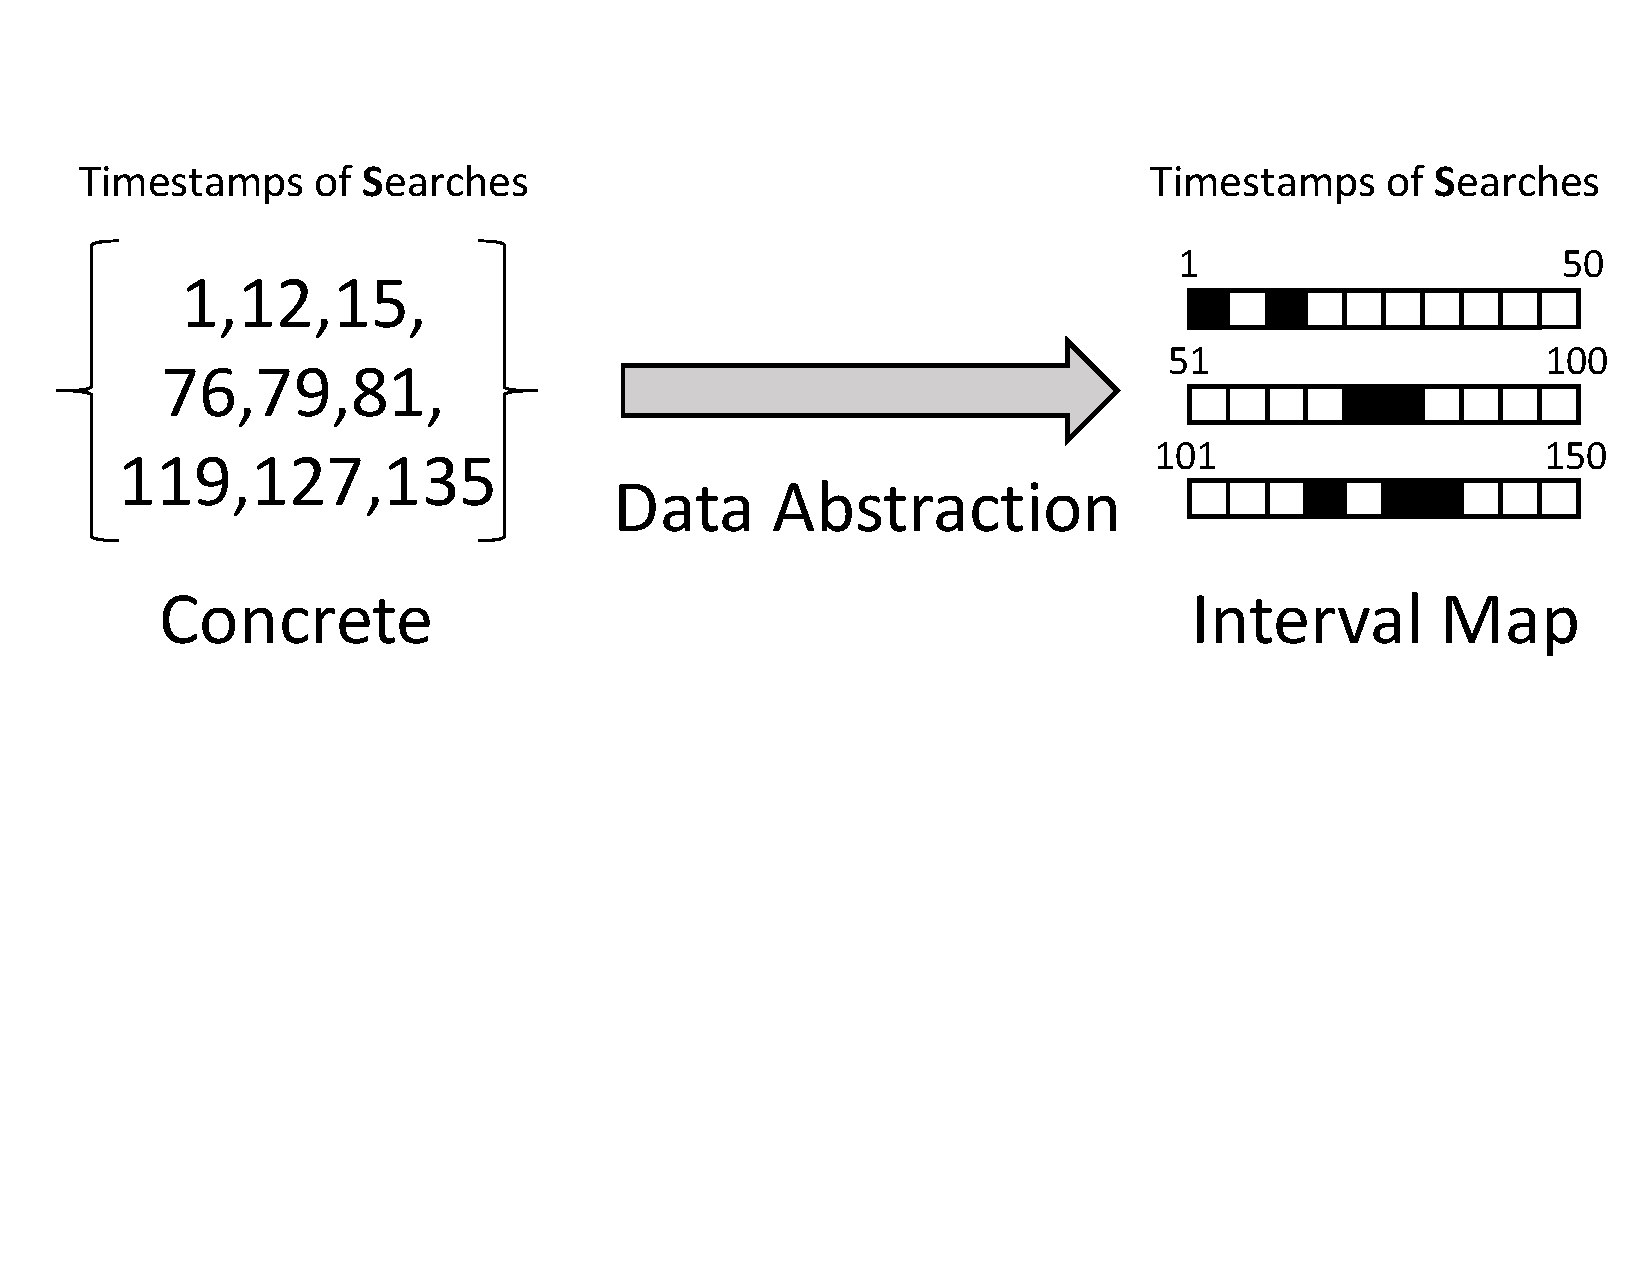
\includegraphics[clip, page=1,width=\columnwidth]{graphs/motivation.pdf}
    \vspace{-3cm}
    \caption{Intervals are a compact over-approximation of users that search.}
    \label{fig:dabstraction}
  \end{subfigure}
  %
  \begin{subfigure}{\columnwidth}
    \includegraphics[clip, page=2,width=\columnwidth]{graphs/motivation.pdf}
    \caption{SR+P will only match those users that search, possibly read at
      least one review, and finally, purchase a product.  Predicate abstraction
      exploits the selectivity of one predicate (most users do not purchase) to
      efficiently over-approximate users that match SR+P.}
    \label{fig:pabstraction}
  \end{subfigure}
\end{figure}
      
 
Our approach is inspired by the concept of abstract 
interpretation~\cite{Cousot:1977,Graf:1997}.  
In particular, the {\em abstract filter} constraints are the result of
relaxing/coarsening in a conservative manner of the precise constraints enforced
by the pattern regarding which events form successful matches.  This suggests
future work can leverage the technique of abstract interpretation to optimize
other user defined operators as well, (i.e.\ to derive abstract filters meant to
remove from the input those tuples that are guaranteed not to contribute to an
output of interest).

% abstract interpretation provides a template for how  this optimization can be 
%extended to other udf running in the reducer stages of a map-reduce pipeline 

%(Results)
As previously mentioned, constructing and applying the abstract filter incurs a
series of overheads, most notably it requires a second pass over the data.
Nonetheless, if the reduction in data is significant, these additional costs are
balanced out by the dramatic speedup in the sorting/shuffling/pattern matching
phases which results in an overall decrease in both processing costs and
latency.  Our experimental evaluation shows up to 3 orders of magnitude
reduction in shuffled data as well as 1.23x average speedup in total processing
time for 2 workloads: i) telemetry analysis over the events produced by an
event-reporting infrastructure, and ii) repository analysis over the dataset of
events published by GitHub.  The reduction in total processing time is
especially important in multi-tenant clusters where clients are billed based on
the amount of computational resources they consume.

The contributions of this paper are:
\begin{itemize}
	\item We show how a significant class of complex event patterns can be 
	translated to relational queries such that they can benefit from decades of 
	progress in relational optimizations.
	\item We introduce the technique of {\em abstract pattern matching} in 
	order to minimize the sorting/shuffling costs of large scale mining of 
	patterns within map-reduce frameworks.
	\item We highlight how the concepts of symbolic execution and abstract 
	interpretation can be used to design similar optimizations for other 
	user-defined reduce operators.
	\item We prototype our solution and show on an industrial benchmark that 
	it delivers significant reductions in the amount of data sorted/shuffled as 
	well as processing times.  
\end{itemize}


The rest of the paper is organized as follows: we discuss related work in the 
next section, then we further illustrate our approach and detail its design in 
sections~\ref{sec:mot_example} and~\ref{sec:design}. 
The choices we made in implementing our solution are explored in 
section~\ref{sec:implementation}, followed by the presentation of the results 
of our experimental evaluation in section~\ref{sec:evaluation}. 
Finally, section~\ref{sec:conclusions} gives our concluding remarks and 
comments on future directions.   


